\documentclass[conference]{IEEEtran}
\IEEEoverridecommandlockouts
% ---------------------------------------------------------------
% Auto EA-SORAN: A Safety-Gated AI-Native Closed-Loop Energy
% Optimization Framework for 5G RANs in a Simu5G Digital Twin.
%
% CURRENT-STATE REVIEW DRAFT.
% All quantitative claims correspond to the matched seed-42 pilot
% only. Multi-seed statistical validation has NOT yet been done.
% Figures are taken verbatim from the current repository outputs.
% ---------------------------------------------------------------
\usepackage{cite}
\usepackage{amsmath,amssymb,amsfonts}
\usepackage{algorithmic}
\usepackage{graphicx}
\usepackage{textcomp}
\usepackage{xcolor}
\usepackage{array}
\graphicspath{{figures/}}
\def\BibTeX{{\rm B\kern-.05em{\sc i\kern-.025em b}\kern-.08em
    T\kern-.1667em\lower.7ex\hbox{E}\kern-.125emX}}
\begin{document}

\title{Auto EA-SORAN: A Safety-Gated AI-Native Closed-Loop Energy Optimization Framework for 5G RANs in a Simu5G Digital Twin}

\author{\IEEEauthorblockN{1\textsuperscript{st} Given Name Surname}
\IEEEauthorblockA{\textit{dept. name of organization} \\
\textit{name of organization}\\
City, Country \\
email address or ORCID}
\and
\IEEEauthorblockN{2\textsuperscript{nd} Given Name Surname}
\IEEEauthorblockA{\textit{dept. name of organization} \\
\textit{name of organization}\\
City, Country \\
email address or ORCID}
\and
\IEEEauthorblockN{3\textsuperscript{rd} Given Name Surname}
\IEEEauthorblockA{\textit{dept. name of organization} \\
\textit{name of organization}\\
City, Country \\
email address or ORCID}
}

\maketitle

% ===============================================================
\begin{abstract}
The energy consumption of fifth-generation (5G) Radio Access Networks (RANs) is a growing operational and environmental concern, motivating autonomous, data-driven energy control. This paper presents Auto EA-SORAN (Autonomous Energy-Aware Self-Optimizing Radio Access Network), an Artificial Intelligence (AI)-native closed-loop control framework that continuously monitors, predicts, optimizes, and validates the energy configuration of a 5G RAN modeled inside a Simu5G digital twin. The loop couples four cooperating agents---a Prediction Agent, an Optimization Agent, a Feedback/Safety Agent, and an Orchestration Agent---that communicate with the Simu5G C++ side over ZeroMQ (ZMQ) inter-process messaging, while a load-coupled analytical gNodeB (gNB) energy model provides the represented-energy signal used for evaluation. A Feedback/Safety Agent enforces policy guard rails and supports rollback so that only safe actions reach the simulated radio. We report a single matched seed (seed 42) pilot on a 30-gNB, 90-User-Equipment (UE) topology driven by a compressed 24-hour logical traffic profile. In this pilot the AI controller reduced represented energy from 54.36 kWh to 50.58 kWh, a 6.95\% Energy Saving (ES), while aggregate throughput changed by only $-0.006\%$ and data Energy Efficiency (EE) improved by approximately 7.46\%. The improvement was accompanied by measurable Quality of Service (QoS) trade-offs: traffic-weighted latency, aggregate packet loss, and Physical Resource Block (PRB) utilization all increased. SHapley Additive exPlanations (SHAP) analysis of the energy predictor is used to interpret which input features drive the energy estimate. These results establish end-to-end feasibility of safety-gated AI-native RAN energy control but remain a single-seed pilot; multi-seed statistical validation is future work.
\end{abstract}

\begin{IEEEkeywords}
5G, RAN energy efficiency, AI-native networks, closed-loop control, digital twin, Simu5G, multi-agent systems, energy saving, explainable AI, SHAP, QoS trade-off
\end{IEEEkeywords}

% ===============================================================
\section{Introduction}
Fifth-generation (5G) New Radio (NR) networks deliver substantially higher capacity than previous generations, but at the cost of dense deployments and increased per-site processing. Although a 5G Base Station (BS) is more energy-efficient per bit than its predecessors, the aggregate energy consumption of a deployed network is larger because more cells are required to provide coverage at higher frequencies and wider bandwidths. The Radio Access Network (RAN), and in particular the gNodeB (gNB) radio units, dominates this energy footprint. Reducing RAN energy without degrading the Quality of Service (QoS) experienced by User Equipment (UE) is therefore a central problem for sustainable network operation.

Energy saving in the RAN is fundamentally a control problem: configuration parameters such as transmit power, bandwidth, carrier count, and Energy-Saving (ES) modes (for example light sleep, sleep, carrier shutdown, and bandwidth-part adaptation) must be adjusted in response to time-varying traffic, while respecting operator policies and Service Level Agreements (SLAs). Traditional rule-based Self-Organizing Network (SON) and Operations, Administration, and Maintenance (OA\&M) mechanisms encode static thresholds and cannot easily exploit learned structure in the data. This motivates Artificial Intelligence (AI)-native control, in which Machine Learning (ML) models predict energy behavior and an optimizer searches for favorable configurations inside a closed loop.

This paper presents \textbf{Auto EA-SORAN} (Autonomous Energy-Aware Self-Optimizing Radio Access Network), an AI-native closed-loop framework for RAN energy optimization that runs against a Simu5G digital twin. Its design contributions are: (i) a four-agent closed loop---Prediction, Optimization, Feedback/Safety, and Orchestration---in which Python agents communicate with the Simu5G C++ side over ZeroMQ (ZMQ) Inter-Process Communication (IPC); (ii) a Feedback/Safety Agent that validates each candidate against policy guard rails and supports rollback, so that only safe actions are physically applied to controllable gNB state; (iii) a load-coupled analytical gNB energy model that produces the \emph{represented energy} signal used for evaluation; and (iv) an explainability layer based on SHapley Additive exPlanations (SHAP) for the energy predictor.

We deliberately frame the experimental contribution as a \emph{pilot}. The results reported here come from a single matched random seed (seed 42) on a 30-gNB, 90-UE topology, evaluated over a compressed 24-hour logical traffic profile. In this matched pilot, AI control reduced represented energy by 6.95\% with practically unchanged throughput, but with measurable latency, packet-loss, and Physical Resource Block (PRB) utilization trade-offs. We do not claim statistical significance, real-world hardware energy measurement, production readiness, or that every Key Performance Indicator (KPI) improved. The contribution is an honest, reproducible demonstration of feasibility together with a clear statement of what remains to be validated.

% ===============================================================
\section{Related Work and Background}
\textbf{Standardized energy metrics.} The 3rd Generation Partnership Project (3GPP) defines 5G performance measurements in Technical Specification (TS) 28.552 and 5G end-to-end KPIs, including network Energy Efficiency (EE), in TS 28.554 \cite{b_28554,b_28552}. EE is expressed as delivered data volume divided by energy consumption over the same measurement period (bit/J). The 3GPP SA5 working group and associated energy-efficiency activities provide the conceptual basis for treating energy saving as a measurable, standardized objective \cite{b_3gpp_ee}. Auto EA-SORAN adopts these definitions: it reports represented energy, average power, throughput, and a data-per-energy EE consistent with the NG-RAN form, while making explicit that its energy figure is analytically represented rather than metered on hardware.

\textbf{System-level simulation and energy modeling.} Simu5G is an OMNeT++/INET-based system-level simulator for 5G NR that models the gNB--UE radio stack and supports discrete-event evaluation of RAN behavior \cite{b_simu5g}. The INET framework additionally provides reference power-consumption and energy-storage models for networked nodes \cite{b_inet}. In this work Simu5G acts as the digital twin: it generates genuine traffic and radio KPIs, exposes controllable gNB transmit power and ES state, and applies orchestrated configuration changes, while a load-coupled analytical model converts radio activity into a represented-energy signal.

\textbf{AI/ML for 5G energy modeling.} Data-driven energy modeling of 5G base stations was the subject of the International Telecommunication Union (ITU) AI/ML in 5G Challenge on 5G energy-consumption modeling, in which base-station energy was estimated from configuration, traffic, and ES-method features \cite{b_itu}. Auto EA-SORAN reuses an Artificial Neural Network (ANN) energy predictor derived from that line of work as its Prediction Agent, and embeds it inside a closed control loop rather than using it only for offline estimation.

\textbf{Explainability.} SHAP provides a unified, game-theoretic framework for additive feature attribution that assigns each input feature a contribution to a model's output \cite{b_shap}. We apply SHAP to the energy predictor to rank the features that most influence the predicted energy, which supports transparency of the AI-native control decisions.

% ===============================================================
\section{System Architecture}
Auto EA-SORAN is organized as a closed control loop around the Simu5G digital twin. Genuine runtime signals from the simulator are collected by a telemetry agent, processed by an energy predictor, optimized subject to policy constraints, validated for safety, and finally applied back to the controllable gNB state. The end-to-end path is:
\begin{quote}\small
Simu5G runtime signals $\rightarrow$ TwinMetricsAgent $\rightarrow$ ZMQ telemetry $\rightarrow$ Prediction Agent $\rightarrow$ Optimization Agent $\rightarrow$ rules or AI healing $\rightarrow$ Feedback/Safety Agent $\rightarrow$ Orchestration Agent $\rightarrow$ OrchestrationShim $\rightarrow$ ControllableGnbPhy $\rightarrow$ physical Simu5G state.
\end{quote}

\subsection{Prediction Agent}
The Prediction Agent hosts a Keras/TensorFlow ANN energy predictor. It subscribes to the Simu5G telemetry stream, maps simulator fields (for example \texttt{prb\_util\_pct}, \texttt{tx\_power\_dbm}, \texttt{es\_mode}) onto the model's engineered feature space, predicts per-cell energy for the current configuration, and forwards the predictions to the Optimization Agent. The 30 cells in the topology are predicted as a single batch to keep inference well below the logical decision interval.

\subsection{Optimization Agent}
The Optimization Agent searches the configuration space---transmit power, bandwidth, carrier count, and ES modes---for low-energy operating points subject to policy constraints. It uses bounded population-based search (evolutionary optimization) and policy retrieval to propose candidate configurations. A candidate is only forwarded when its predicted energy saving exceeds a minimum-benefit threshold, which prevents low-value configuration churn.

\subsection{Feedback/Safety Agent}
The Feedback/Safety Agent is the safety gate of the architecture. It validates each proposed configuration against operator and standards-aligned policies, computes a policy-compliance score, counts critical violations, and either approves or rejects the plan. Rejected or violating plans trigger rollback to a known-safe configuration. This agent is the mechanism by which the framework restricts the applied action set to a safe subset (Section~\ref{sec:math}), and is the reason the system can pursue energy reduction without silently violating QoS policy.

\subsection{Orchestration Agent and Simu5G Coupling}
The Orchestration Agent translates an approved plan into a command for the C++ OrchestrationShim, which actuates the ControllableGnbPhy module inside Simu5G. The orchestration reply reports both the \emph{requested} and the \emph{physically applied} state---transmit power, bandwidth, carrier count, sleep state, cell index, and the simulation time at which the change took effect. This acknowledgement is important methodologically: it ensures that a reported saving reflects a change that actually reached the simulator, not a Python-side decision alone. Transmit power and the supported ES state are physically applied to the simulated gNB PHY; some additional configuration dimensions are represented analytically within the energy model (Section~\ref{sec:limitations}).

% ===============================================================
\section{Methodology and Implementation}
\subsection{Digital twin and topology}
The digital twin is a 30-gNB, 90-UE Simu5G NR network with three UEs associated around each gNB. The 30 cells are organized into a Bangalore-inspired multi-zone layout (for example central business district macro cells, information-technology park cells, and residential cells), each zone carrying a distinct daily traffic shape and radio-unit profile. This 30-cell configuration was chosen as a credible city-scale research pilot that remains executable on a development laptop.

\subsection{Compressed logical day}
A full 24-hour traffic cycle is represented in 60 seconds of physical simulation time, using a logical time scale of 1440 logical seconds per physical second ($60$ physical seconds $= 86{,}400$ logical seconds $= 24$ hours). This compression makes repeated experiments feasible while retaining the intended daily sequence of \emph{very-low}, \emph{low}, \emph{medium}, and \emph{peak} traffic conditions; the simulator still executes every scheduled discrete event. The compression does not imply real-time execution.

\subsection{Compared control strategies}
Two strategies are compared on identical network and traffic conditions. The \emph{deterministic} strategy keeps monitoring and energy prediction active but selects ES actions from operator-defined rules, without the AI healing path or Feedback/Safety Agent action selection. The \emph{AI} strategy processes telemetry through the ANN predictor, searches for energy-saving configurations with the Optimization Agent, optionally refines a healing plan, validates it with the Feedback/Safety Agent, and applies the approved plan through the Orchestration Agent. A minimum-benefit guard rejects candidates whose predicted energy saving is below $0.5\%$.

\subsection{Inter-process communication}
All four Python agents and the Simu5G C++ side communicate over ZMQ sockets (publish/subscribe for telemetry and request/reply for control), forming the IPC backbone of the loop. Predictions are drained in bounded batches and feedback polling is non-blocking, so that telemetry processing does not stall under load.

\subsection{Evaluation matching}
Because the two collectors can start one snapshot apart, raw runs are temporally matched before comparison. The paper-facing matched set covers physical simulation time 4\,s through 60\,s, with 57 common snapshots, 30 cells per snapshot (1{,}710 cell rows per scenario), seed 42, replicate 1, and no unassociated UEs. All headline values in this paper use this common matched window.

% ===============================================================
\section{Mathematical Formulation}\label{sec:math}
\subsection{Load-coupled gNB power model}
Represented per-gNB power is produced by a load-coupled analytical model. In its general linear-in-load form,
\begin{equation}
P_{\mathrm{gNB}}(t) = P_{\mathrm{idle}} + \alpha\, u_{\mathrm{PRB}}(t), \label{eq:linear}
\end{equation}
where $P_{\mathrm{idle}}$ is the load-independent static power, $u_{\mathrm{PRB}}(t) \in [0,1]$ is the instantaneous PRB utilization (load), and $\alpha$ scales the dynamic, traffic-coupled component. The implemented model refines \eqref{eq:linear} with explicit static, dynamic, antenna, baseband, and carrier terms,
\begin{equation}
\begin{aligned}
P_{\mathrm{gNB}} = \big( & P_{\mathrm{static}} + \delta\,P_{\max}\, u_{\mathrm{PRB}}\, s_{\mathrm{bw}}\, s_{\mathrm{cc}}\, s_{\mathrm{tx}} \\
& + P_{\mathrm{ant}} + P_{\mathrm{bb}} + P_{\mathrm{cc}} \big)\, \eta\, m_{\mathrm{es}},
\end{aligned}\label{eq:fullpower}
\end{equation}
where $\delta$ is the dynamic-power coefficient, $P_{\max}$ the maximum dynamic power, and $s_{\mathrm{bw}}$, $s_{\mathrm{cc}}$, $s_{\mathrm{tx}}$ are bandwidth, carrier-count, and transmit-power scaling factors respectively (with $s_{\mathrm{tx}}$ following a $10^{(P_{\mathrm{tx}}-P_{\mathrm{tx,base}})/10}$ law). The terms $P_{\mathrm{ant}}$, $P_{\mathrm{bb}}$, and $P_{\mathrm{cc}}$ capture antenna, baseband, and additional-carrier power, $\eta$ is a cooling/auxiliary overhead factor, and $m_{\mathrm{es}}\le 1$ is the multiplicative saving applied by the active ES mode (for example sleep, light sleep, carrier-off, MIMO reduction, micro-DTX, or bandwidth-part adaptation). This is the load-coupled analytical gNB energy model; it is not a measurement of physical base-station hardware energy.

\subsection{Represented energy over time}
Represented energy is accumulated over the evaluated interval as
\begin{equation}
E = \sum_{t=1}^{T} P(t)\,\Delta t \;\;\equiv\;\; \int_{0}^{T} P(t)\,dt, \label{eq:energy}
\end{equation}
where each physical measurement interval $\Delta t$ represents a longer logical interval, and the same represented interval is used for both scenarios after matching. Energy is reported in kWh by dividing the joule total by $3.6\times10^{6}$.

\subsection{Energy saving}
The headline energy saving is the relative reduction of represented energy from the deterministic baseline to the AI configuration,
\begin{equation}
\Delta E\,(\%) = \frac{E_{\mathrm{base}} - E_{\mathrm{opt}}}{E_{\mathrm{base}}}\times 100, \label{eq:es}
\end{equation}
where $E_{\mathrm{base}}$ is the baseline (deterministic) represented energy and $E_{\mathrm{opt}}$ is the optimized (AI) represented energy.

\subsection{Energy efficiency}
Following the standardized data-energy form, EE is performance per unit energy,
\begin{equation}
EE = \frac{\mathrm{Performance}}{\mathrm{Energy}} \;\;\longrightarrow\;\; EE = \frac{\mathrm{Throughput}}{E}, \label{eq:ee}
\end{equation}
reported here as represented received data volume (Mbit) divided by represented energy (J), i.e. Mbit/J. This is consistent with the NG-RAN data-EE definition in 3GPP TS 28.554, whose standardized unit is bit/J; we use Mbit/J for readability.

\subsection{QoS safety-guard condition}
The Feedback/Safety Agent restricts the applied action $a_t$ to a safe set $\mathcal{A}_{\mathrm{safe}}$ defined by QoS guard rails,
\begin{equation}
a_t \in \mathcal{A}_{\mathrm{safe}} \iff
\begin{cases}
\mathrm{Throughput}_{p95} \ge \theta_{\mathrm{thr}}, \\
\mathrm{Latency}_{p95} \le \theta_{\mathrm{lat}}, \\
\mathrm{Loss}_{p95} \le \theta_{\mathrm{loss}},
\end{cases}\label{eq:safe}
\end{equation}
where $\theta_{\mathrm{thr}}$, $\theta_{\mathrm{lat}}$, and $\theta_{\mathrm{loss}}$ are policy thresholds on tail throughput, latency, and packet loss. Only actions that satisfy these guard rails (and the policy-compliance and critical-violation checks) are approved; otherwise the agent rejects the plan and rolls back. The percentiles and thresholds are configurable policy parameters.

\subsection{Optimization objective}
The controller objective is to minimize represented energy subject to QoS constraints,
\begin{equation}
\min_{a_t \in \mathcal{A}} \; E_t(a_t)
\quad \text{s.t.} \quad \mathrm{QoS}_i(a_t) \le \theta_i, \;\; \forall i, \label{eq:obj}
\end{equation}
with the additional minimum-benefit constraint that a candidate is applied only when its predicted saving relative to the current configuration exceeds the guard threshold ($0.5\%$). Equation~\eqref{eq:obj} is realized by the Optimization Agent's search, while the constraints in \eqref{eq:safe} are enforced by the Feedback/Safety Agent.

\subsection{Predictor attribution}
For the energy predictor $f$, SHAP expresses a prediction as an additive feature attribution,
\begin{equation}
f(x) = \phi_0 + \sum_{i=1}^{M} \phi_i, \label{eq:shap}
\end{equation}
where $\phi_0$ is the base (expected) prediction and $\phi_i$ is the contribution of feature $i$. For global importance, features are ranked by their mean absolute SHAP value $\frac{1}{n}\sum_{j} |\phi_i^{(j)}|$ across the explained cohort, which orders features by their average influence on the predicted energy.

% ===============================================================
\section{Experimental Setup}
The experiment compares the deterministic and AI strategies on the matched seed-42 window described above: 30 gNBs, 90 UEs, 57 common snapshots over physical time 4--60\,s, representing a full logical 24-hour traffic cycle with very-low, low, medium, and peak regimes. The Prediction Agent uses the Keras ANN energy predictor; the Optimization Agent uses bounded evolutionary search with policy retrieval; the Feedback/Safety Agent enforces policy and the minimum-benefit guard; and the Orchestration Agent applies approved changes to controllable gNB transmit power and ES state in Simu5G. KPIs are computed with the represented-energy, throughput, EE, latency, packet-loss, PRB-utilization, and sleeping-cell-time formulas summarized in Section~\ref{sec:math}, aggregated across cells and represented intervals. Confidence-interval fields exist in the analysis outputs but are zero because only one run per scenario is present; they are not statistical error bars and are not interpreted as evidence of low variance.

% ===============================================================
\section{Results and Discussion}
\subsection{Headline matched results}
Table~\ref{tab:headline} reports the matched seed-42 KPIs. The AI controller reduced represented energy from 54.36\,kWh to 50.58\,kWh, a 6.946\% energy saving by \eqref{eq:es}, and reduced average network power by approximately 165.6\,W. Aggregate throughput changed by only $-0.006\%$, so delivered traffic was practically preserved. Consequently, data energy efficiency improved from 0.028076 to 0.030170\,Mbit/J, about $+7.46\%$ by \eqref{eq:ee}. These gains were not free: traffic-weighted latency rose from 2.933 to 3.934\,ms, aggregate packet loss rose from 0.000629\% to 0.006290\% (a small absolute increase), PRB utilization rose from 2.458\% to 3.332\%, and full-sleep cell-time rose from 2.749\% to 3.099\%. The associated-UE population was unchanged at 90. We therefore describe the outcome as an energy/QoS trade-off observed in the matched seed-42 experiment, not as a uniform improvement of all KPIs.

\begin{table}[htbp]
\caption{Matched Seed-42 Pilot KPIs (Deterministic vs. AI). Single Matched Seed; Not Statistically Conclusive.}
\begin{center}
\renewcommand{\arraystretch}{1.15}
\begin{tabular}{|l|r|r|r|}
\hline
\textbf{KPI} & \textbf{Determ.} & \textbf{AI} & \textbf{Change} \\
\hline
Represented energy (kWh) & 54.3601 & 50.5842 & $-6.946\%$ \\
\hline
Avg.\ network power (W) & 2384.21 & 2218.60 & $-165.6$\,W \\
\hline
Avg.\ throughput (Mbit/s) & 66.9394 & 66.9356 & $-0.006\%$ \\
\hline
Energy efficiency (Mbit/J) & 0.028076 & 0.030170 & $+7.46\%$ \\
\hline
Traffic-wtd.\ latency (ms) & 2.933 & 3.934 & $+34.1\%$ \\
\hline
Aggregate packet loss (\%) & 0.000629 & 0.006290 & $+0.00566$\,pp \\
\hline
Weighted PRB util.\ (\%) & 2.458 & 3.332 & $+0.874$\,pp \\
\hline
Sleeping cell-time (\%) & 2.749 & 3.099 & $+0.350$\,pp \\
\hline
Avg.\ associated UEs & 90 & 90 & unchanged \\
\hline
\end{tabular}
\label{tab:headline}
\end{center}
\end{table}

\subsection{KPI comparison}
Fig.~\ref{fig:kpi} shows the multi-panel KPI comparison. The lower AI energy and power bars confirm the energy reduction, while the near-identical throughput bars show preserved traffic delivery and the higher AI EE bar shows more data delivered per joule. The higher AI latency and packet-loss bars expose the QoS trade-off. The pattern is consistent with the controller consolidating traffic onto fewer active radio resources and operating them more intensively, which lowers energy but raises tail latency, loss, and PRB utilization. Because only one run per scenario is present, the figure carries no statistical error bars.

\begin{figure}[htbp]
\centerline{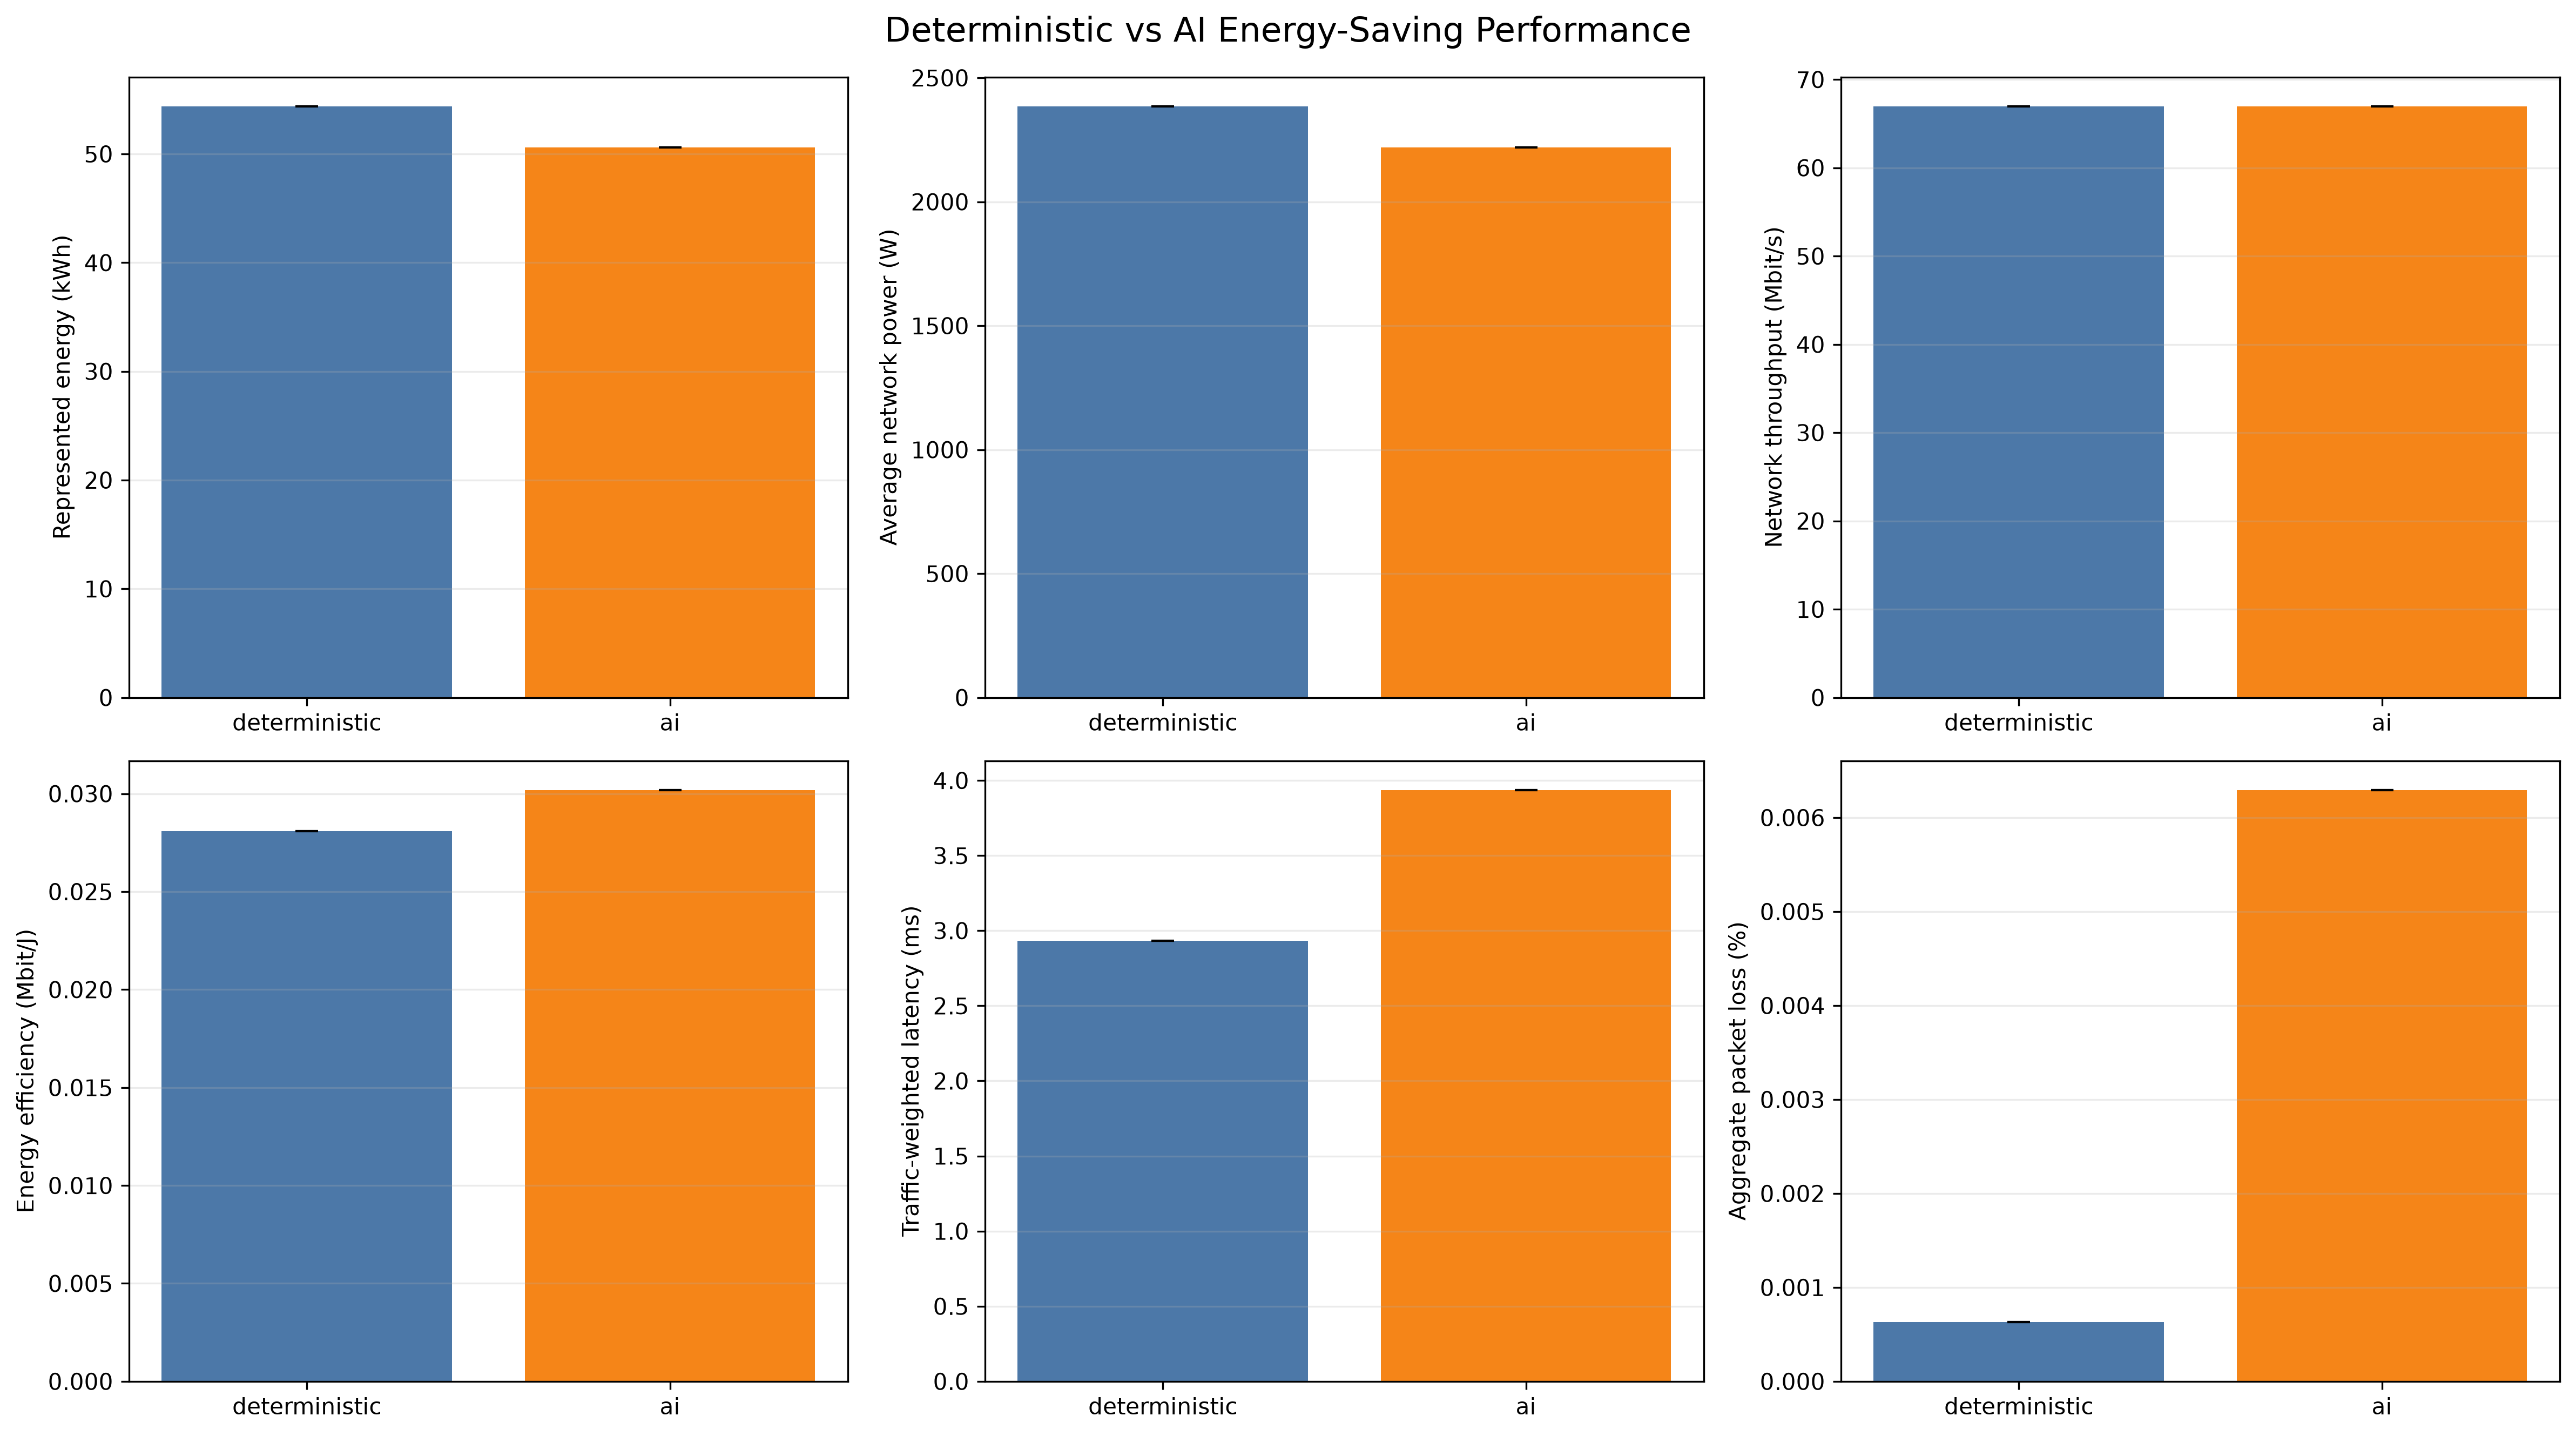
\includegraphics[width=\columnwidth]{kpi_comparison.png}}
\caption{Matched seed-42 KPI comparison (deterministic vs.\ AI). Energy and power decrease and energy efficiency increases, while throughput is nearly flat; latency, packet loss, and PRB utilization worsen. Single-seed pilot: bars carry no statistical error bars.}
\label{fig:kpi}
\end{figure}

\subsection{Energy--throughput trade-off}
Fig.~\ref{fig:tradeoff} places the two scenarios in energy--throughput space. The AI operating point moves toward lower energy without moving materially toward lower throughput, which is the favorable direction for energy efficiency and supports the EE improvement in \eqref{eq:ee}. With a single seed, the plot contains one point per scenario and should be read as a pilot visualization rather than a statistically characterized frontier.

\begin{figure}[htbp]
\centerline{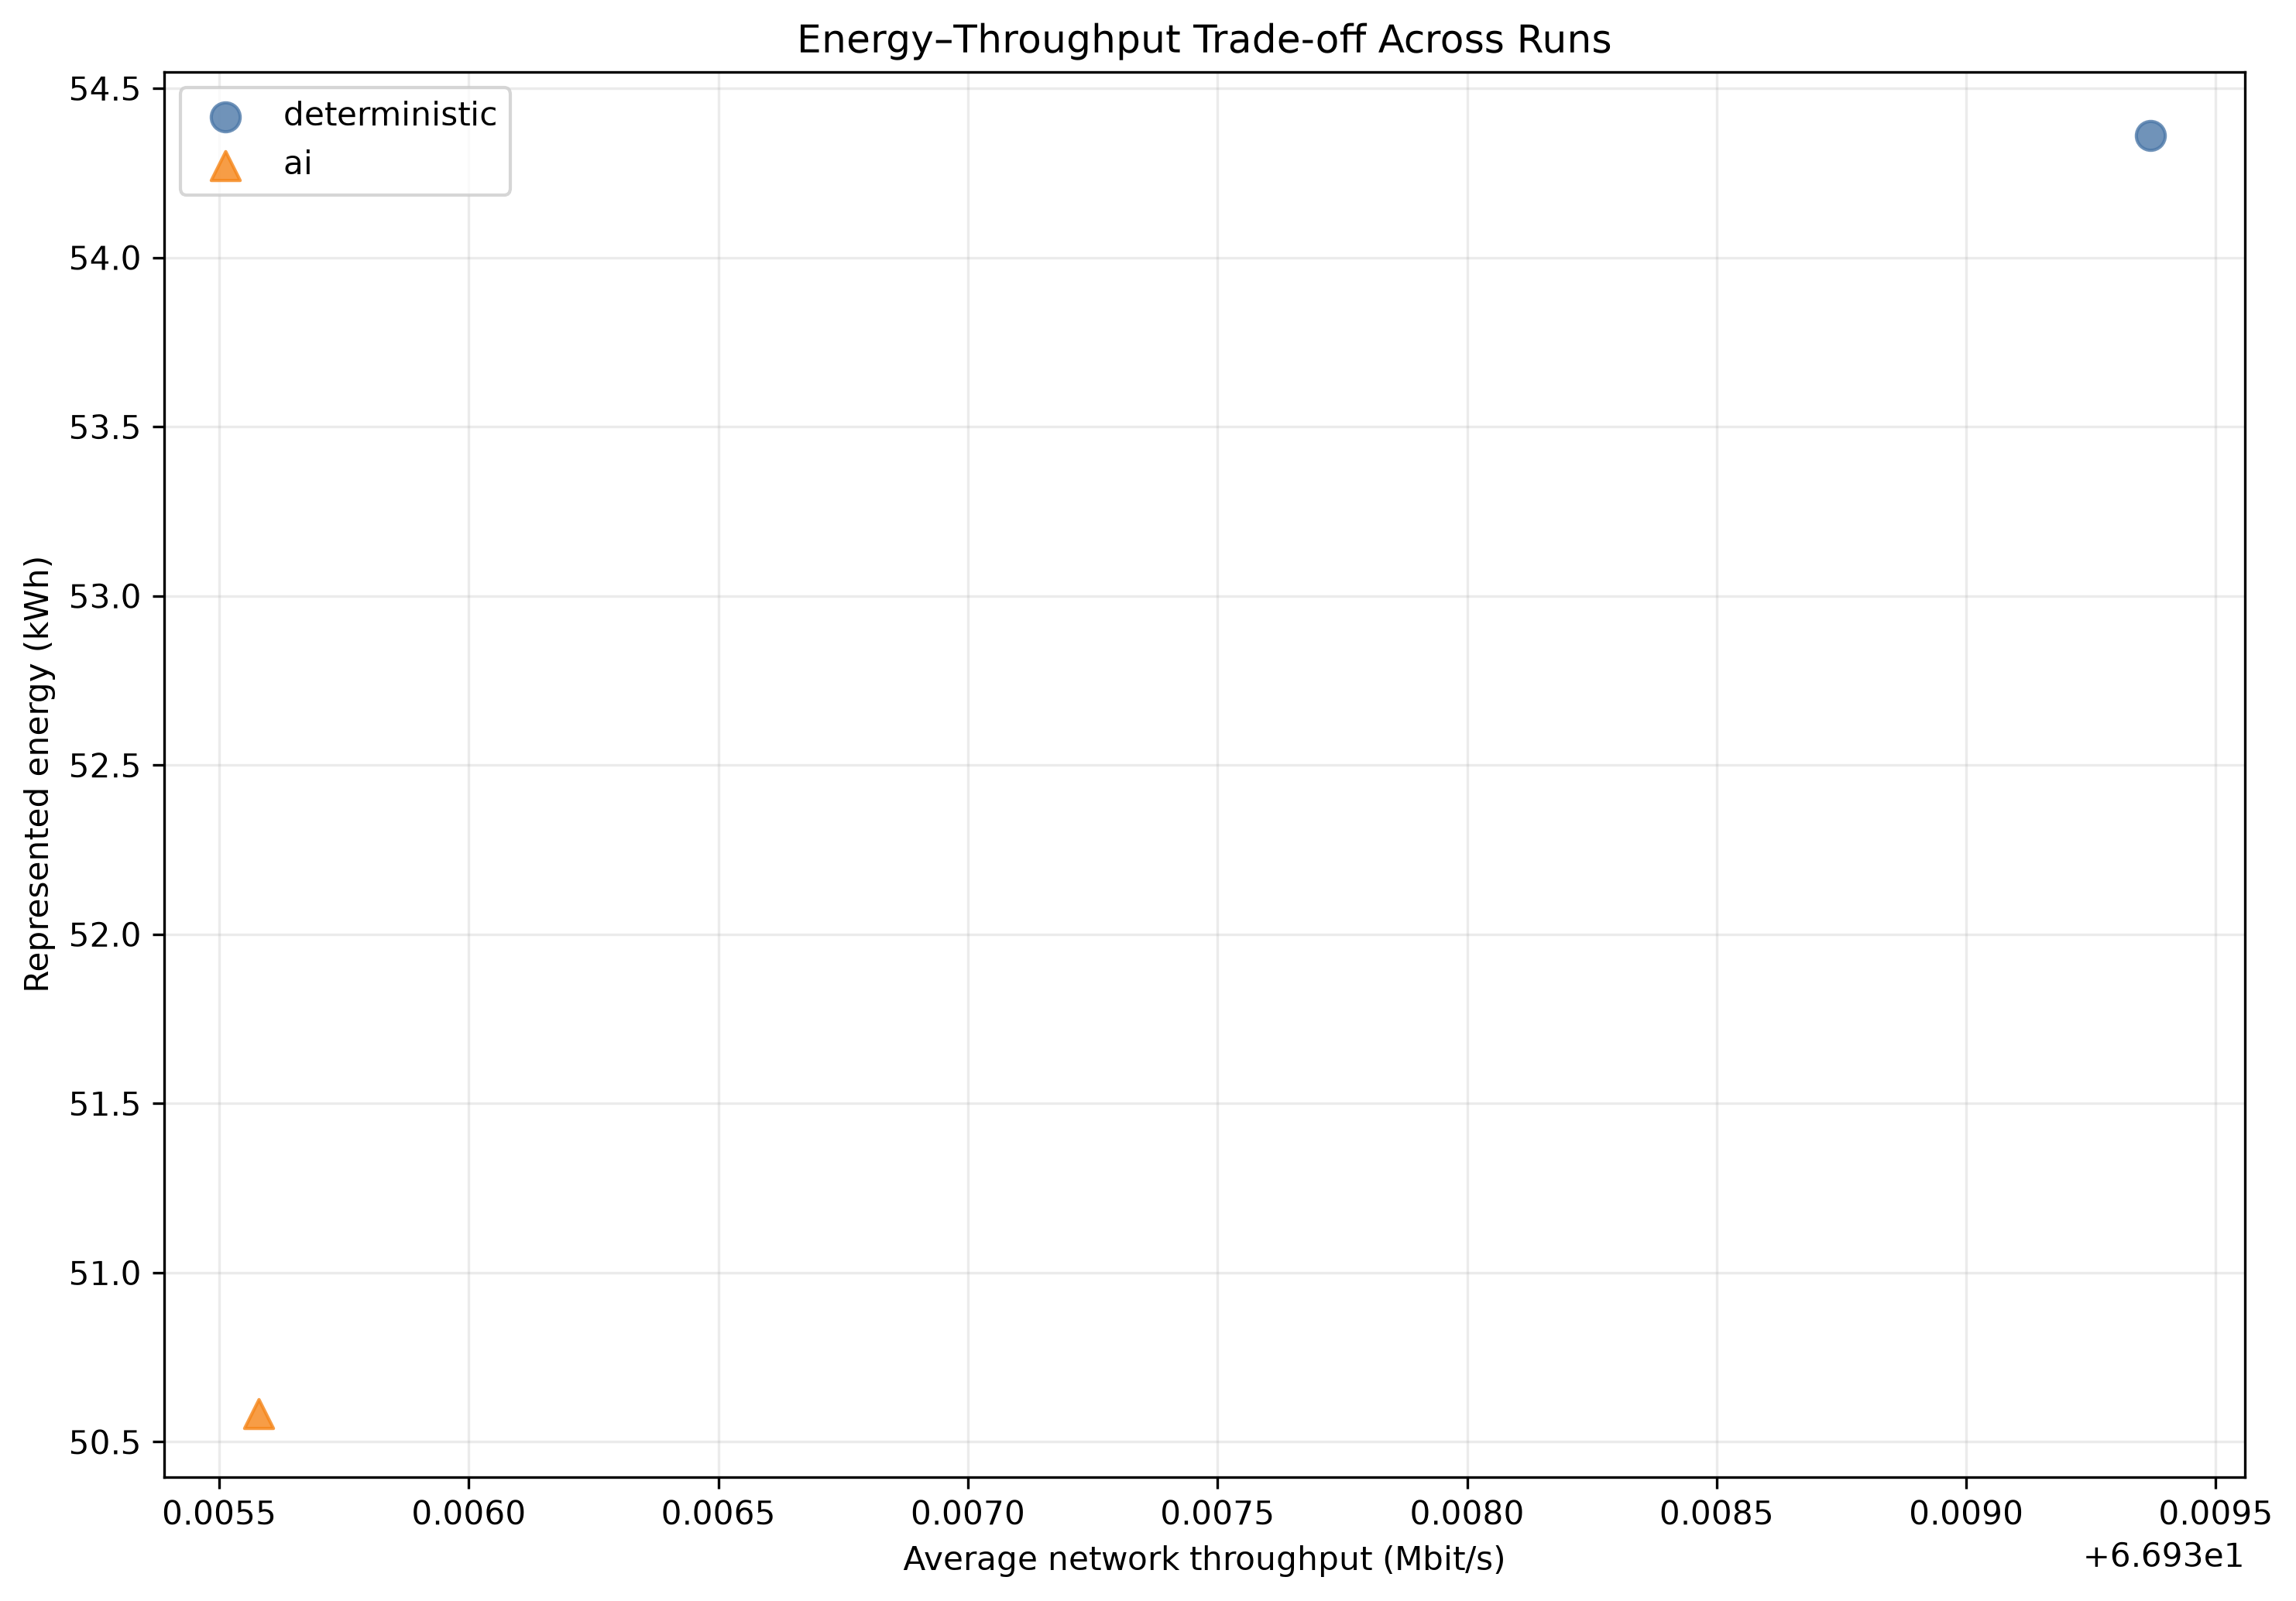
\includegraphics[width=\columnwidth]{energy_throughput_tradeoff.png}}
\caption{Energy--throughput trade-off for the matched seed-42 pilot. The AI point sits at lower energy with practically unchanged throughput, supporting the energy-efficiency claim. One point per scenario; pilot visualization only.}
\label{fig:tradeoff}
\end{figure}

\subsection{Temporal behavior over the logical day}
Fig.~\ref{fig:hourly} shows network power, throughput, PRB utilization, and latency across the compressed 24-hour logical day. It is the primary figure for relating control behavior to the daily traffic cycle: power broadly tracks demand, and the AI controller has the most freedom to reduce power during low-load periods, where it acts most aggressively. Consolidation during these periods is also where latency and PRB utilization tend to rise. Table~\ref{tab:bytraffic} quantifies the saving by traffic regime: the largest saving (8.558\%) occurs at very-low traffic, where the controller can transition the most radio resources, while positive savings are retained even at peak (5.562\%) under service-protection constraints.

\begin{figure}[htbp]
\centerline{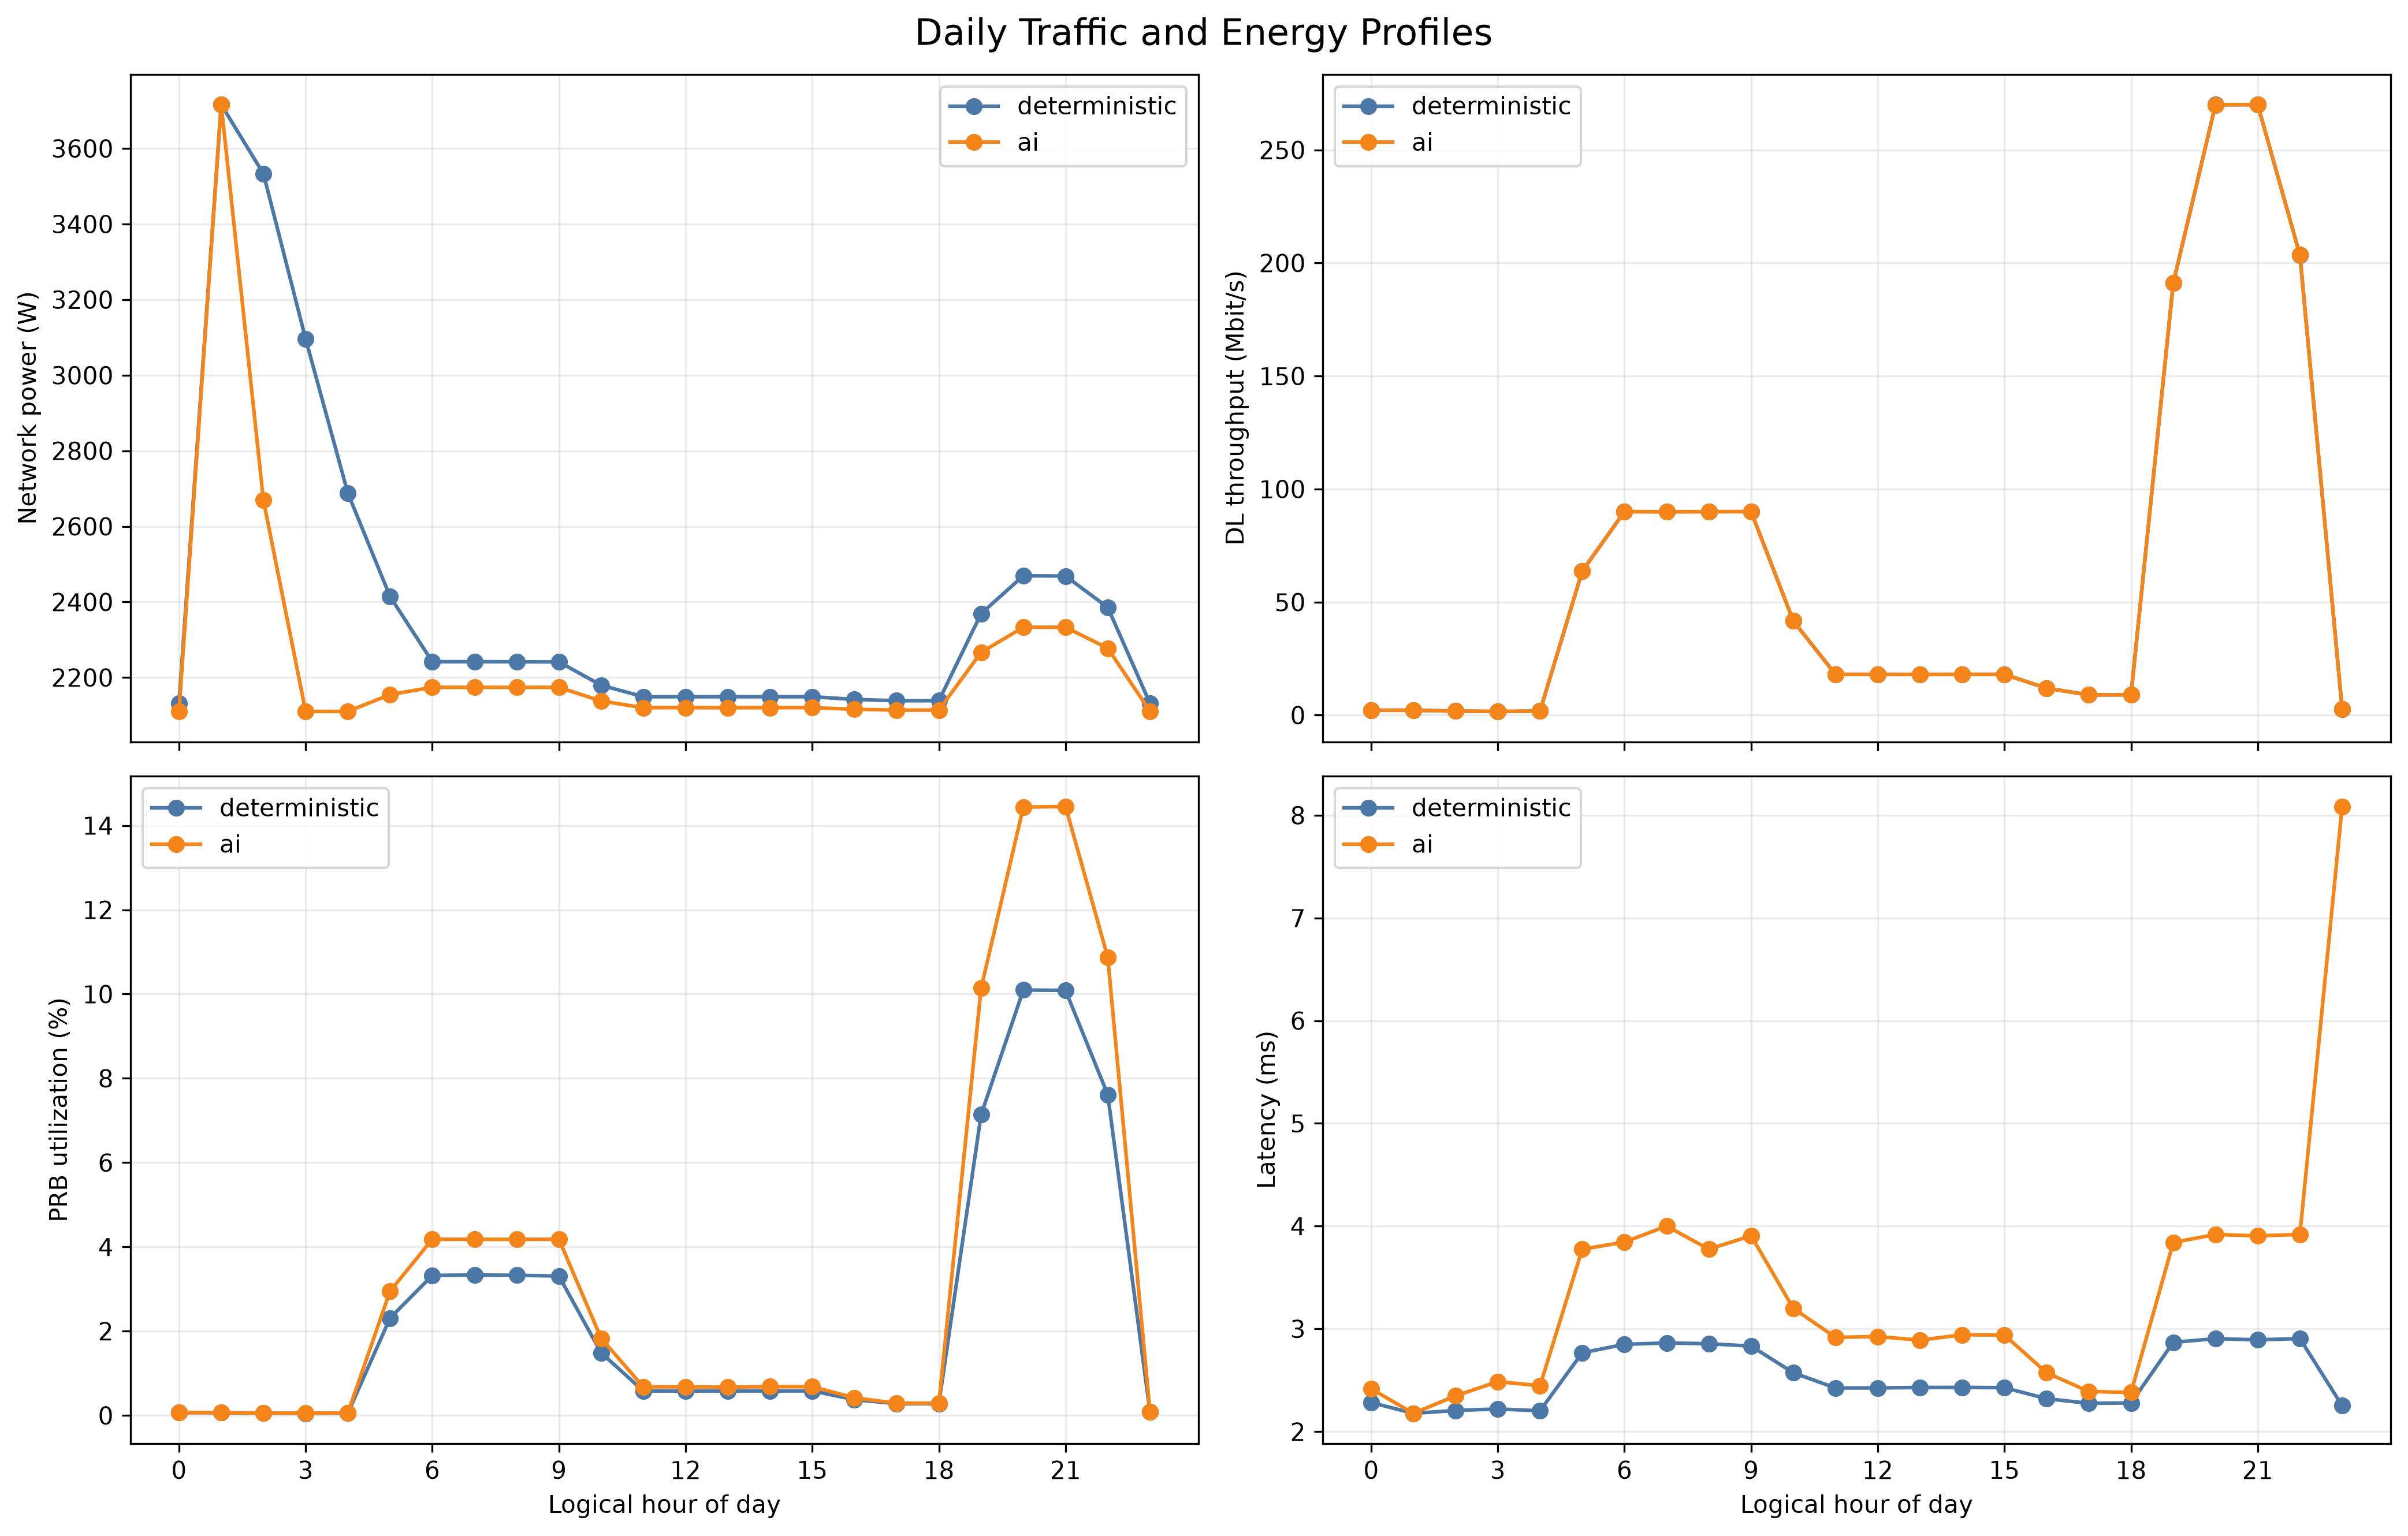
\includegraphics[width=\columnwidth]{hourly_profiles.png}}
\caption{Representative temporal behavior over the logical 24-hour day (power, throughput, PRB utilization, latency). Power follows demand; the controller saves most during low-load periods, where consolidation also raises latency and PRB utilization. Matched seed-42 pilot.}
\label{fig:hourly}
\end{figure}

\begin{table}[htbp]
\caption{AI Energy Saving by Traffic Regime (Matched Seed 42)}
\begin{center}
\renewcommand{\arraystretch}{1.1}
\begin{tabular}{|l|r|}
\hline
\textbf{Traffic regime} & \textbf{Energy saving vs.\ deterministic} \\
\hline
Very low & 8.558\% \\
\hline
Low & 3.444\% \\
\hline
Medium & 3.191\% \\
\hline
Peak & 5.562\% \\
\hline
\end{tabular}
\label{tab:bytraffic}
\end{center}
\end{table}

\subsection{Energy-saving modes by traffic}
Fig.~\ref{fig:esmodes} reports the share of represented cell-time spent in each \emph{applied} ES mode by traffic regime. In the AI run, light sleep dominates (1{,}587 of 1{,}710 cell observations, 92.81\%), with a smaller active share (70, 4.09\%) and a full-sleep share (53, 3.10\%); the deterministic run kept more observations active (211) and used light sleep less (1{,}452). All low, medium, and peak observations were served by light sleep, while the full-sleep and remaining active observations occurred during very-low traffic. This indicates that the policy protected availability under higher demand and reserved the deepest transitions for the lowest-load period. The chart shows only \emph{applied} configurations: candidate modes such as bandwidth-part adaptation or micro-DTX are absent because they did not pass the minimum-benefit guard in this run, which is a deployment constraint and not evidence that those modes are universally ineffective.

\begin{figure}[htbp]
\centerline{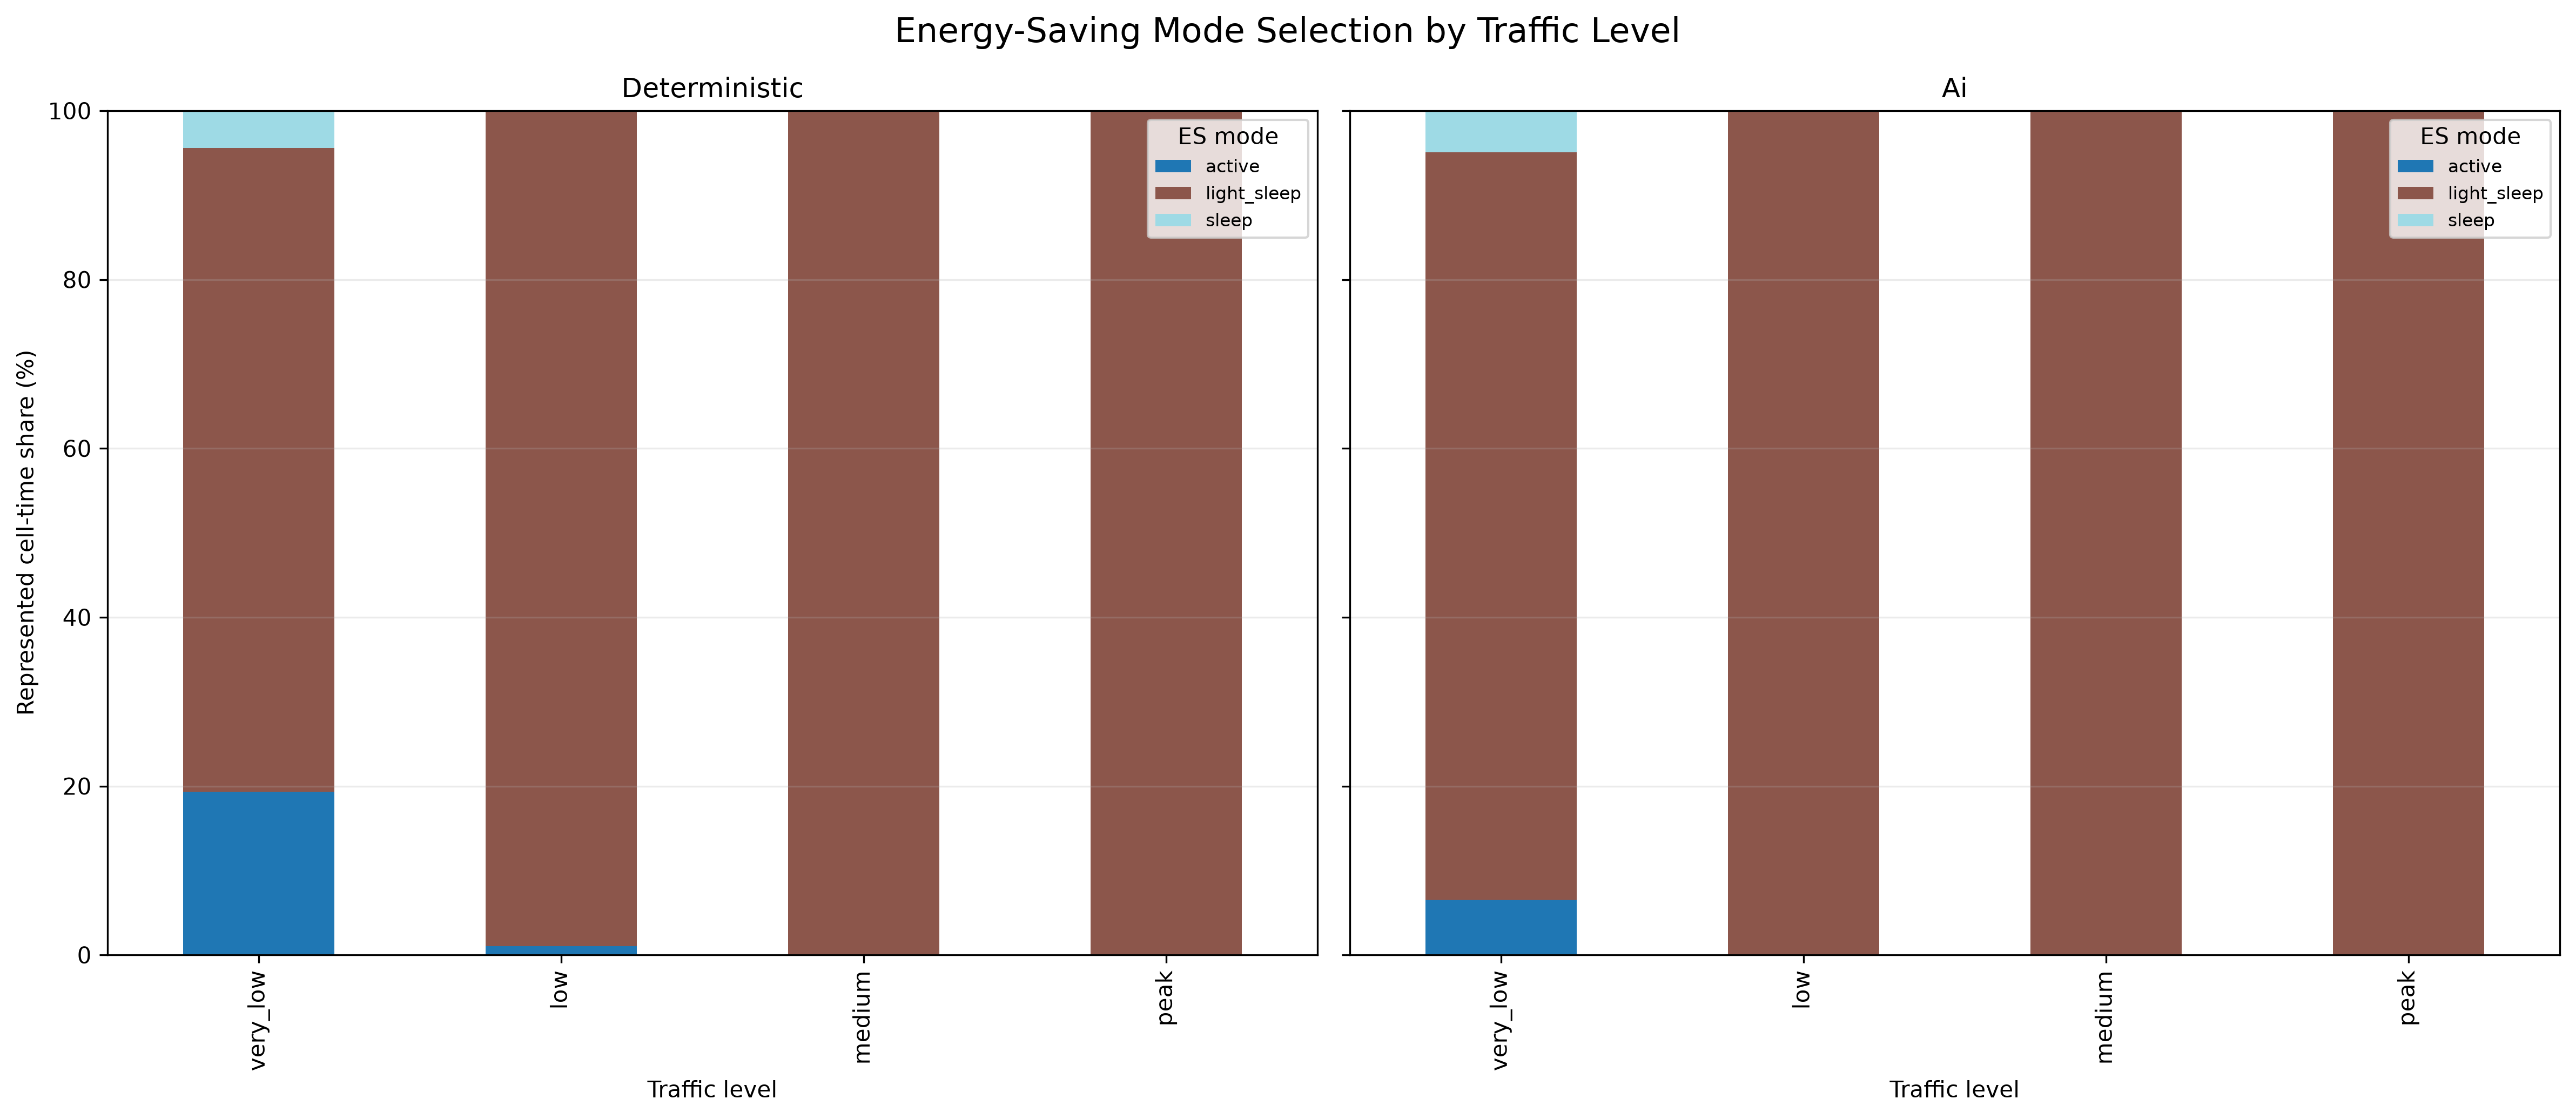
\includegraphics[width=\columnwidth]{es_modes_by_traffic.png}}
\caption{Applied energy-saving mode distribution by traffic regime (matched seed-42 AI run). Light sleep dominates across all regimes; full sleep is reserved for very-low traffic. Modes rejected by the minimum-benefit guard are intentionally absent.}
\label{fig:esmodes}
\end{figure}

\subsection{Global explainability of the energy predictor}
Fig.~\ref{fig:shap} ranks the energy predictor's input features by mean absolute SHAP value (Equation~\eqref{eq:shap}). The most influential features are the time-of-day spline components (notably \texttt{hour\_spline\_2} and \texttt{hour\_spline\_1}), configured bandwidth, the smoothed load and load-spline features, weekday/day features, and transmit power. This is consistent with the physics of the energy model: energy is driven by time-coupled traffic (load and time-of-day), by bandwidth and transmit power through the dynamic-power scaling in \eqref{eq:fullpower}, and by the daily/weekly seasonality of demand. The ranking supports the interpretability of the AI-native loop by showing that the predictor relies on operationally meaningful, traffic- and configuration-related features rather than on spurious inputs. SHAP here explains the energy predictor only; it does not explain the rule engine, the policy logic, or the multi-agent system as a whole.

\begin{figure}[htbp]
\centerline{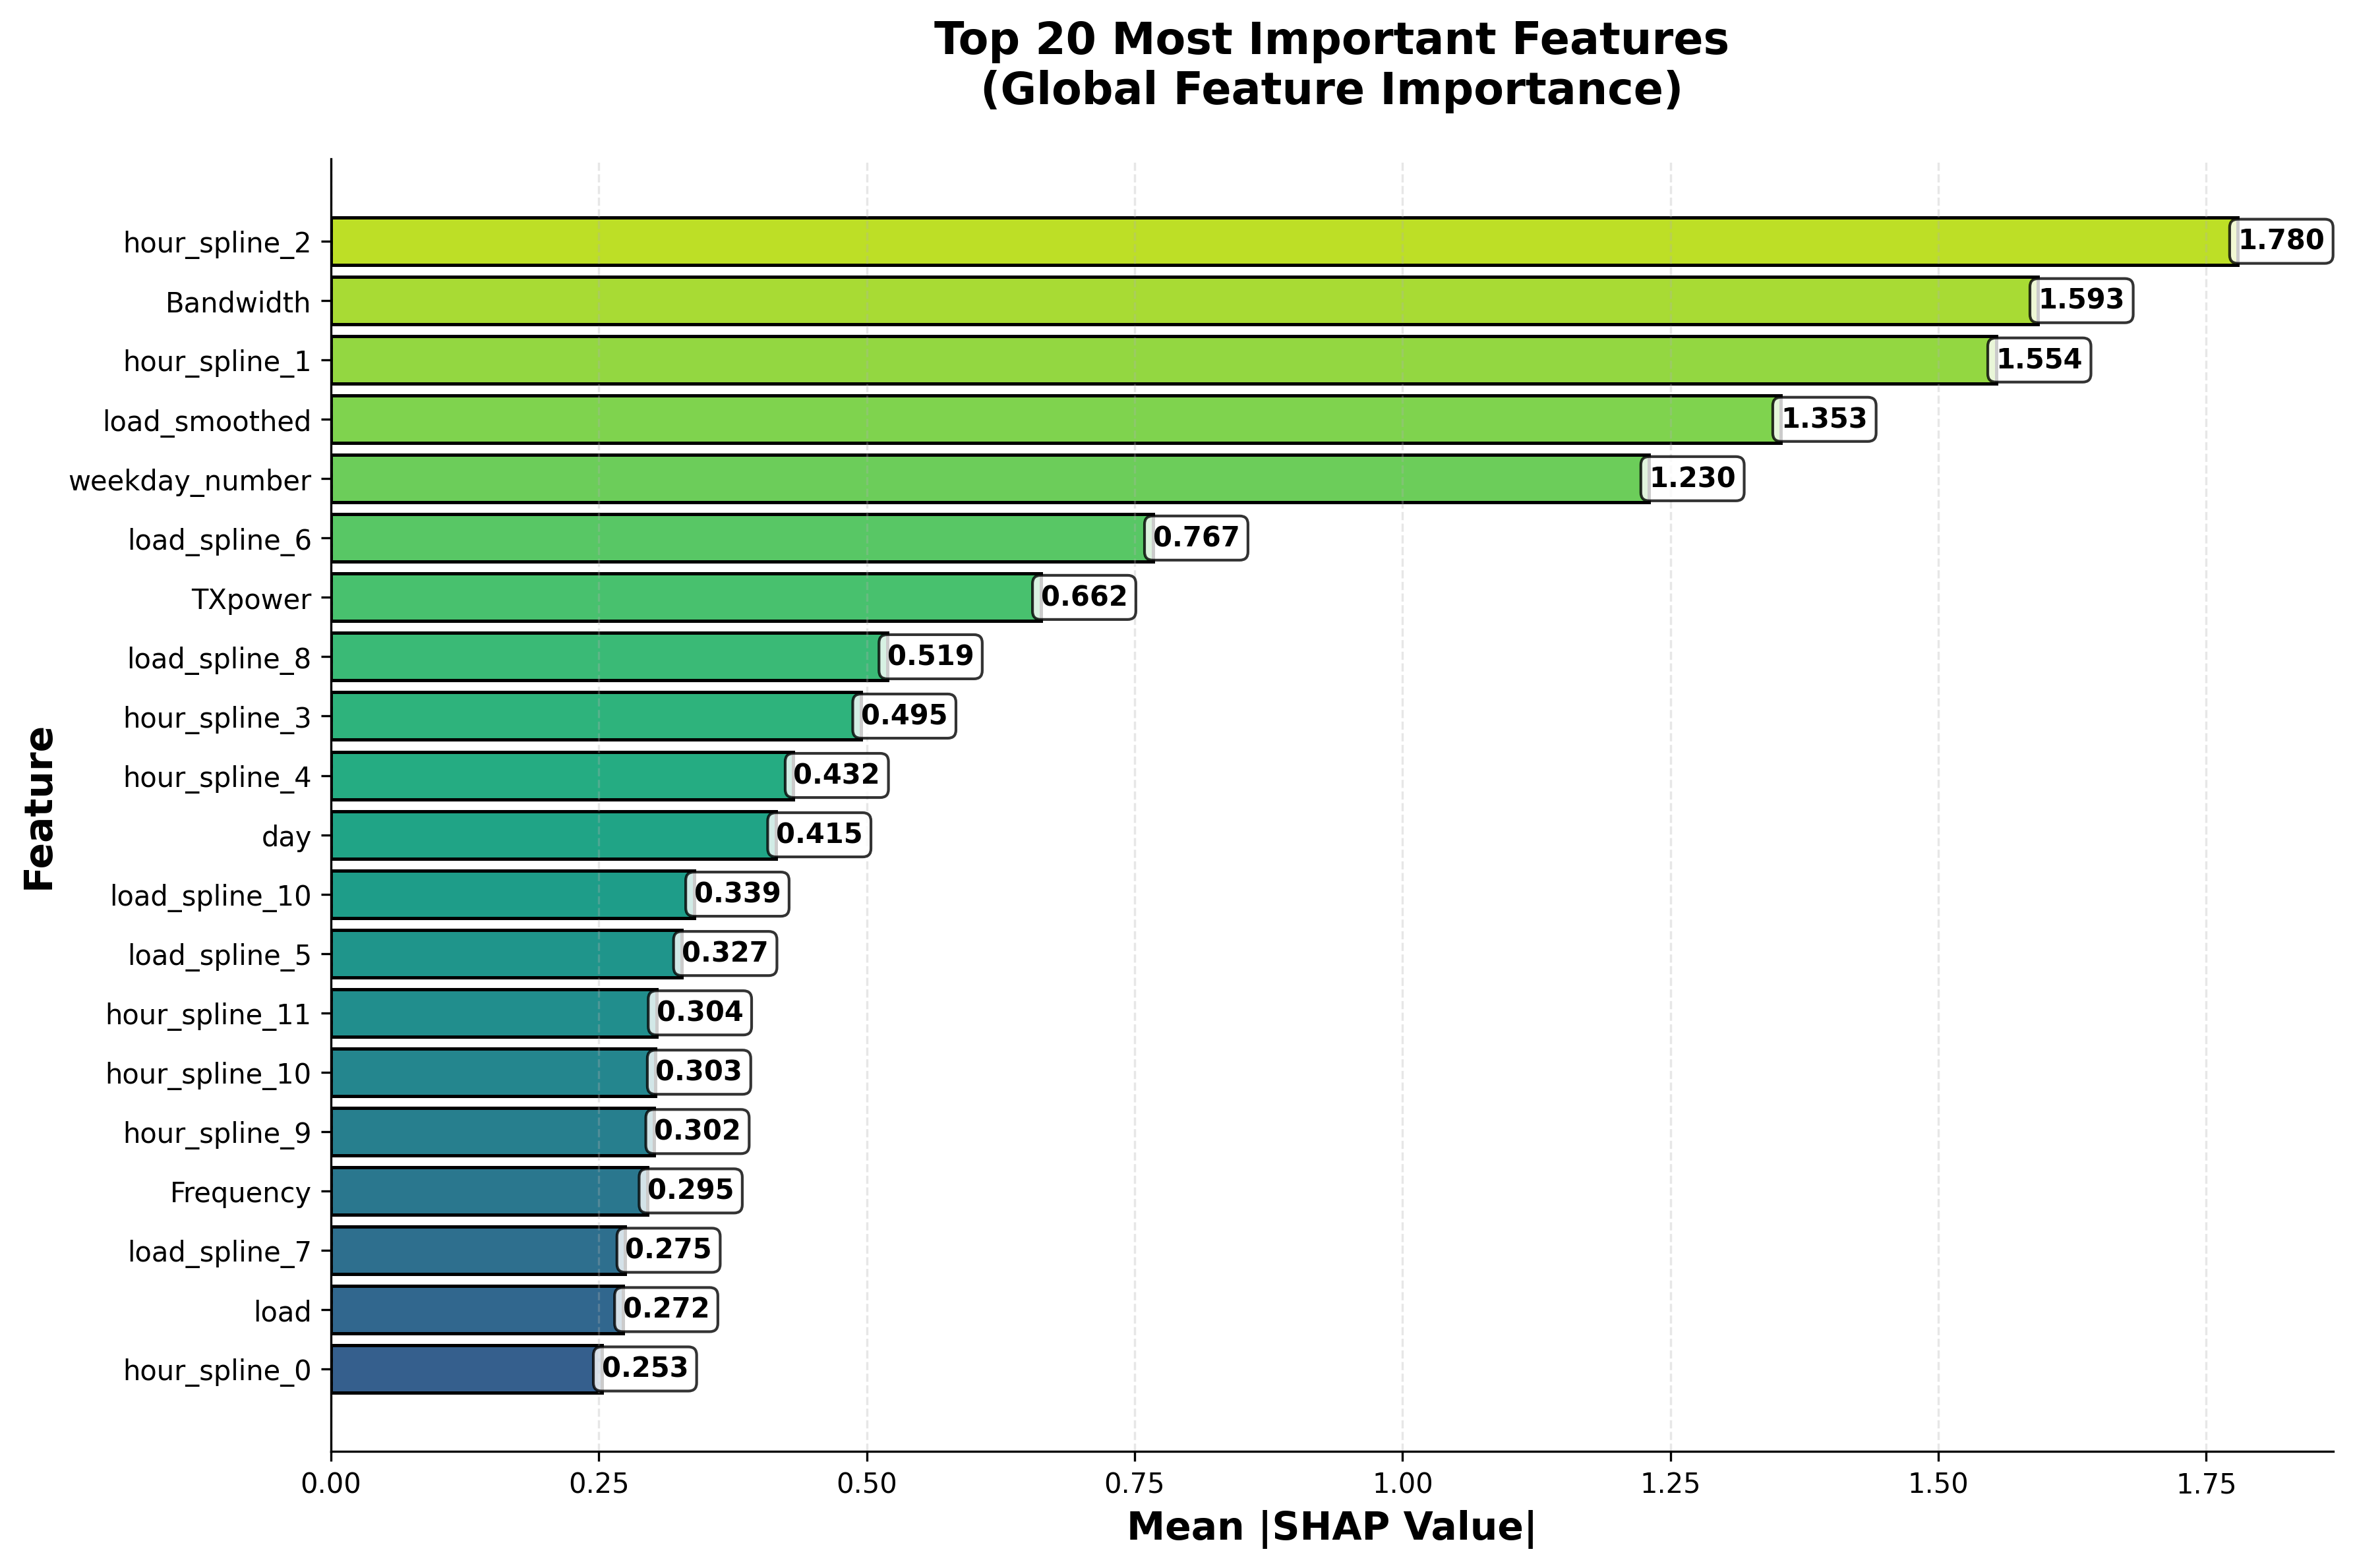
\includegraphics[width=\columnwidth]{shap_explanation_1_importance_bar.png}}
\caption{Global feature importance of the energy predictor by mean absolute SHAP value. Time-of-day spline features, bandwidth, smoothed load/load-spline features, weekday/day features, and transmit power dominate, consistent with the load-coupled energy model. SHAP explains the predictor only.}
\label{fig:shap}
\end{figure}

\subsection{Discussion}
Taken together, the matched seed-42 pilot suggests that safety-gated AI-native control can reduce represented RAN energy by a meaningful margin (about 6.95\%) while preserving throughput, at the cost of bounded and measurable increases in latency, packet loss, and PRB utilization. The Feedback/Safety Agent and minimum-benefit guard are central to this behavior: they keep deeper transitions out of high-load regimes and prevent low-value churn, so the energy gain is obtained within policy guard rails. We emphasize that these observations come from a single matched seed and should be read as a feasibility result, not as a statistically conclusive performance claim.

% ===============================================================
\section{Limitations}\label{sec:limitations}
We state the limitations explicitly. First, all results derive from a \emph{single matched seed} (seed 42); statistical generalization requires multi-seed validation, and no significance is claimed. Second, energy is \emph{represented} through a load-coupled analytical gNB model (Equations~\eqref{eq:linear}--\eqref{eq:fullpower}), not measured on physical base-station hardware; the values are not commercial power-meter readings. Third, the actuation is partial: transmit power and the supported ES state are physically applied to the controllable gNB PHY, while some configuration dimensions (for example bandwidth, frequency, antenna count, and radio-unit type) are represented analytically or held at defaults rather than fully actuated in the simulator. Fourth, the comparison currently includes only a deterministic rule baseline; stronger baselines are needed---no-control, static-threshold, AI-without-feedback, and AI-without-rollback---to attribute the gain precisely. Fifth, more traffic regimes and longer simulations are needed beyond the compressed single-day pilot. Sixth, a more detailed QoS tail analysis (percentile latency and loss distributions) is needed to characterize the trade-off fully. None of these limitations invalidates the feasibility demonstration, but each bounds the strength of the present claims.

% ===============================================================
\section{Future Work}
The immediate priority is statistical validation: at least a 10-seed evaluation per scenario with reported means, standard deviations, 95\% confidence intervals, paired effect sizes, and significance testing. We further plan stronger baselines (no-control, static-threshold, deterministic, AI-without-feedback, AI-without-rollback) and targeted ablation studies that isolate the contribution of the Feedback/Safety Agent and the rollback mechanism. We will enrich actuator support so that more configuration dimensions are physically applied in Simu5G, extend the topology and add multi-cell coordination, and evaluate additional and longer traffic regimes. We also intend to align the control loop with O-RAN and the near-Real-Time RAN Intelligent Controller (RIC) so that the agents can be expressed as xApps, and to deepen the explainability analysis (local explanations and stability of the SHAP rankings across seeds).

% ===============================================================
\section{Conclusion}
We presented Auto EA-SORAN, a safety-gated AI-native closed-loop framework for 5G RAN energy optimization built around a Simu5G digital twin, in which Prediction, Optimization, Feedback/Safety, and Orchestration agents cooperate over ZMQ and a load-coupled analytical model provides the represented-energy signal. In a matched seed-42 pilot on a 30-gNB, 90-UE topology over a compressed 24-hour traffic cycle, AI control reduced represented energy by 6.95\% with practically unchanged throughput and an approximately 7.46\% improvement in data energy efficiency, while incurring measurable latency, packet-loss, and PRB-utilization trade-offs. The Feedback/Safety Agent and rollback mechanism kept the controller within policy guard rails, and SHAP analysis confirmed that the energy predictor relies on operationally meaningful features. These results demonstrate end-to-end feasibility of safe AI-native RAN energy control; they remain a single-seed pilot, and multi-seed statistical validation with stronger baselines is the essential next step.

% ===============================================================
\begin{thebibliography}{00}
\bibitem{b_28554} 3GPP, ``Management and orchestration; 5G end to end Key Performance Indicators (KPI),'' 3GPP TS 28.554 (ETSI TS 128 554), Release 18. [Online]. Available: https://www.etsi.org/deliver/etsi\_ts/128500\_128599/128554/
\bibitem{b_28552} 3GPP, ``Management and orchestration; 5G performance measurements,'' 3GPP TS 28.552 (ETSI TS 128 552), Release 18. [Online]. Available: https://www.etsi.org/deliver/etsi\_ts/128500\_128599/128552/
\bibitem{b_3gpp_ee} 3GPP, ``Energy efficiency of 5G,'' 3GPP SA5 energy-efficiency overview. [Online]. Available: https://www.3gpp.org/technologies/ee-article
\bibitem{b_simu5g} G. Nardini, D. Sabella, G. Stea, P. Thakkar, and A. Virdis, ``Simu5G--An OMNeT++ library for end-to-end performance evaluation of 5G networks,'' IEEE Access, vol. 8, pp. 181176--181191, 2020.
\bibitem{b_inet} INET Framework, ``Power consumption and energy storage modeling,'' INET Framework documentation. [Online]. Available: https://inet.omnetpp.org/
\bibitem{b_itu} ITU AI/ML in 5G Challenge, ``5G energy consumption modelling,'' International Telecommunication Union, 2023. Solution report, Team Farzi Data Scientists. [Online]. Available: https://aiforgood.itu.int/about-ai-for-good/aiml-in-5g-challenge/
\bibitem{b_shap} S. M. Lundberg and S.-I. Lee, ``A unified approach to interpreting model predictions,'' in Advances in Neural Information Processing Systems (NeurIPS), vol. 30, 2017, pp. 4765--4774.
\end{thebibliography}

\end{document}
